\begin{center}
	{\fboxrule=4pt \fbox{\fboxrule=1pt
		\fbox{\LARGE{\bfseries Enunciado}}}} \\
	\addcontentsline{toc}{section}{Enunciado}
	\rule{15cm}{0pt} \\
\end{center}

\begin{ejer}
    \par El algoritmo de búsqueda de PageRank de Google se basa en el modelo de navegación aleatoria, que es una caminata aleatoria en el gráfico de la web. 
    Para este gráfico, cada vértice representa una página de Internet. Una arista dirigida conecta $i$ con $j$ si hay un enlace de hipertexto de la página $i$ a la página $j$. 
    Cuando el usuario está en la página $i$, se mueve a una nueva página eligiendo entre los enlaces disponibles en $i$ de manera uniforme y aleatoria.
    \par La siguiente figura \ref{fig:redSimplificada} muestra una red simplificada con siete páginas.
\end{ejer}

 %%% IMAGEN DE RED SIMPLIFICADA %%%
\begin{figure}[H]
	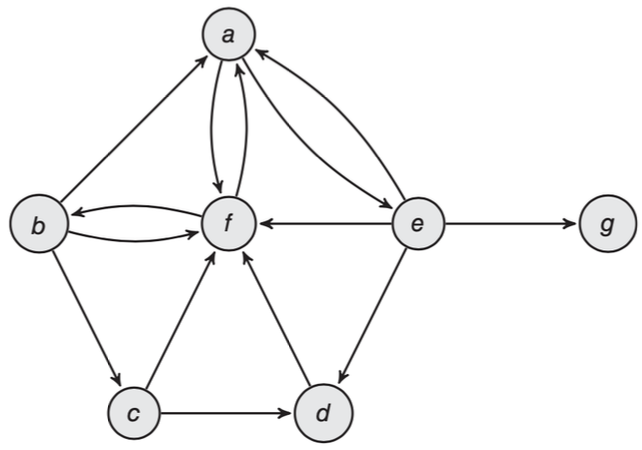
\includegraphics[width=\textwidth/2]{redSimplificada}
	\centering
	\caption{Red Simplificada.}
    \label{fig:redSimplificada}
\end{figure}
\begin{ejer}
    \par La red está descrita por la matriz:
\end{ejer}
%%%% MATRIZ %%%
\begin{equation}
    N =
    \begin{pmatrix}
    0 & 0 & 0 & 0 & 1/2 & 1/2 & 0\\
    1/3 & 0 & 1/3 & 0 & 0 & 1/3 & 0\\
    0 & 0 & 0 & 1/2 & 0 & 1/2 & 0\\
    0 & 0 & 0 & 0 & 0 & 1 & 0 \\
    1/4 & 0 & 0 & 1/4 & 0 & 1/4 & 1/4 \\
    1/2 & 1/2 & 0 & 0 & 0 & 0 & 0 \\
    0 & 0 & 0 & 0 & 0 & 0 & 0 \\
    \end{pmatrix}
    .
\end{equation}

\begin{ejer}
    \par Tenga en cuenta que $N$ no es una matriz estocástica, ya que la página $g$ no tiene enlaces de salida, 
    de modo que la fila asociada a $g$ está formada completamente por ceros (y no suma 1). 
    Para asegurarse de que el camino aleatorio llegua a todas las páginas de la red, el algoritmo debe tener en cuenta (i) 
    las páginas que no tienen enlaces de salida, llamadas nodos colgantes, y (ii) los grupos de páginas que pueden hacer que el camino se atasque en un subgrafo. 
    En la red del ejemplo, $g$ es un nodo colgante. Suponga que la red consta de $k$ páginas. En el algoritmo de PageRank, la solución para los nodos colgantes es 
    asumir que cuando el usuario aleatorio llega a una página de este tipo, salta a una nueva página en la red de manera uniforme y aleatoria.
    Se obtiene una nueva matriz $Q$ donde cada fila de $N$ correspondiente a un nodo colgante se cambia por una en la que todas las entradas son $1/k$. 
    La nueva matriz $Q$ es una matriz estocástica. Para el problema de atascarse potencialmente en pequeños subgrafos de la red, la solución propuesta en el 
    artóculo original por Brin y Page (1998) fue fijar un factor de amortiguamiento $0 < p < 1$ para modificar la matriz $Q$. En su modelo, desde una página dada, 
    el internauta aleatorio, con probabilidad $1 - p$, decide no seguir ningún enlace en la página y, en cambio, navegar a una nueva página aleatoria en la red.
    Por otro lado, con probabilidad $p$, sigue los enlaces de la página como de costumbre. Esto define la matriz de transición de PageRank.
    \par $P =pQ+(1-p)A,$
    \par donde $A$ es una matriz $k x k$ cuyas entradas son todas $1/k$. El factor de amortiguación utilizado por Google se estableció originalmente en $p = 0,85$. 
    Con el factor de amortiguación, la matriz de PageRank $P$ es estocástica y el camino aleatorio resultante es aperiódico e irreducible. 
    El PageRank de una página en la red es la probabilidad estacionaria de esa página.
\end{ejer}